%
% exemplo genérico de uso da classe iiufrgs.cls
% $Id: iiufrgs.tex,v 1.1.1.1 2005/01/18 23:54:42 avila Exp $
%
% This is an example file and is hereby explicitly put in the
% public domain.
%
\documentclass[ppgc,mestrado,english]{iiufrgs}
% um tipo específico de monografia pode ser informado como parâmetro opcional:
%\documentclass[tese]{iiufrgs}
% monografias em inglês devem receber o parâmetro `english':
%\documentclass[diss,english]{iiufrgs}
% a opção `openright' pode ser usada para forçar inícios de capítulos
% em páginas ímpares
% \documentclass[openright]{iiufrgs}
% para gerar uma versão somente-frente, basta utilizar a opção `oneside':
% \documentclass[oneside]{iiufrgs}
\usepackage[T1]{fontenc}        % pacote para conj. de caracteres correto
\usepackage[utf8]{inputenc}   % pacote para acentuação
\usepackage{graphicx}           % pacote para importar figuras
\usepackage{times}              % pacote para usar fonte Adobe Times
\usepackage{mhchem} 	% pacote para usar chemistry formulae
\usepackage{chemfig}
\usepackage{amsmath}
\usepackage{amsthm}
\usepackage{amssymb}
\usepackage{mathtools}
\usepackage{multirow}
\usepackage{acronym}
\usepackage[acronym]{glossaries}
\usepackage{textcomp}
\usepackage{adjustbox}
\usepackage{array}
\usepackage{listings}
\usepackage{tablefootnote}
\usepackage{placeins}


%\usepackage{mathptmx}          % p/ usar fonte Adobe Times nas fórmulas

%
% Informações gerais
%
\title{\emph{SHPECK} - A Geochemical Speciation Modelling Software}

\author{Damiani}{Leonardo Hax}
% alguns documentos podem ter varios autores:
%\author{Flaumann}{Frida Gutenberg}
%\author{Flaumann}{Klaus Gutenberg}

% orientador e co-orientador são opcionais (não diga isso pra eles :))
\advisor[Prof.~Dr.]{Dal Sasso Freitas}{Carla Maria}
\coadvisor[Prof.~Dr.]{Park}{Anthony J.}

% a data deve ser a da defesa; se nao especificada, são gerados
% mes e ano correntes
%\date{maio}{2001}

% o nome do curso pode ser redefinido (ex. para TCs)
%\course{Curso de Especialização em Cachaça}

% o local de realização do trabalho pode ser especificado (ex. para TCs)
% com o comando \location:
%\location{Itaquaquecetuba}{SP}

% itens individuais da nominata podem ser redefinidos com os comandos
% abaixo:
% \renewcommand{\nominataReit}{Prof\textsuperscript{a}.~Wrana Maria Panizzi}
% \renewcommand{\nominataReitname}{Reitora}
% \renewcommand{\nominataPRE}{Prof.~Jos{\'e} Carlos Ferraz Hennemann}
% \renewcommand{\nominataPREname}{Pr{\'o}-Reitor de Ensino}
% \renewcommand{\nominataPRAPG}{Prof\textsuperscript{a}.~Joc{\'e}lia Grazia}
% \renewcommand{\nominataPRAPGname}{Pr{\'o}-Reitora Adjunta de P{\'o}s-Gradua{\c{c}}{\~a}o}
% \renewcommand{\nominataDir}{Prof.~Philippe Olivier Alexandre Navaux}
% \renewcommand{\nominataDirname}{Diretor do Instituto de Inform{\'a}tica}
% \renewcommand{\nominataCoord}{Prof.~Carlos Alberto Heuser}
% \renewcommand{\nominataCoordname}{Coordenador do PPGC}
% \renewcommand{\nominataBibchefe}{Beatriz Regina Bastos Haro}
% \renewcommand{\nominataBibchefename}{Bibliotec{\'a}ria-chefe do Instituto de Inform{\'a}tica}
% \renewcommand{\nominataChefeINA}{Prof.~Jos{\'e} Valdeni de Lima}
% \renewcommand{\nominataChefeINAname}{Chefe do \deptINA}
% \renewcommand{\nominataChefeINT}{Prof.~Leila Ribeiro}
% \renewcommand{\nominataChefeINTname}{Chefe do \deptINT}

% A seguir são apresentados comandos específicos para alguns
% tipos de documentos.

% Relatório de Pesquisa [rp]:
% \rp{123}             % numero do rp
% \financ{CNPq, CAPES} % orgaos financiadores

% Trabalho Individual [ti]:
%\ti{123}     % numero do TI
% \ti[II]{456} % no caso de ser o segundo TI

% Trabalho de Conclusão [tc]:
% além de definir explicitamente o nome do curso (\course) e o local
% de realização (\location), é necessário redefinir a nominata,
% pois as informações necessárias dependem do curso. Ex.:
%\renewcommand{\nominata}{
%        UNIVERSIDADE FEDERAL DO RIO GRANDE DO SUL\\
%        Reitora: Prof\textsuperscript{a}.~Wrana Maria Panizzi\\
%        Pró-Reitor de Ensino: Prof.~José Carlos Ferraz Hennemann\\
%        Diretor do Instituto de Informática: Prof.~Philippe Olivier Alexandre Navaux\\
%        Coordenador do curso: Prof.~Seu Creysson\\
%        Bibliotecária-chefe do Instituto de Informática: Beatriz Regina Bastos Haro
%}

% Monografias de Especialização [espec]:
% \espec{Redes e Sistemas Distribuídos}      % nome do curso
% \coord[Profa.~Dra.]{Weber}{Taisy da Silva} % coordenador do curso
% \dept{INA}                                 % departamento relacionado

%
% palavras-chave
% iniciar todas com letras minúsculas, exceto no caso de abreviaturas
%
\keyword{Geochemical Modelling}
\keyword{Chemical Equilibrium}
\keyword{Geochemical Speciation}
\keyword{Multiphase System}
\keyword{Software Engineering}
\keyword{Computer Science}


%
% inicio do documento
%

\newcolumntype{R}[2]{%
    >{\adjustbox{angle=#1,lap=\width-(#2)}\bgroup}%
    l%
    <{\egroup}%
}
\newcommand*\rot{\multicolumn{1}{R{50}{1em}}}% no optional argument here, please!




\begin{document}



\lstset{language=C++,
	basicstyle=\ttfamily\scriptsize,
	keywordstyle=\color{blue}\ttfamily,
	stringstyle=\color{red}\ttfamily,
	commentstyle=\color{green}\ttfamily,
	breaklines=true}
	
\renewcommand{\lstlistingname}{Code}

% folha de rosto
% às vezes é necessário redefinir algum comando logo antes de produzir
% a folha de rosto:
%\renewcommand{\coordname}{Coordenadora do Curso}
\maketitle

% dedicatoria
\clearpage
\begin{flushright}
\mbox{}\vfill
\end{flushright}

% sumario
\renewcommand*\contentsname{Summary}
\tableofcontents

% lista de abreviaturas e siglas
% o parametro deve ser a abreviatura mais longa


\begin{listofabbrv}{SPMD}
\item[a] Activity
\item[ASCII] American Standard Code For Information Interchange
\item[CRUD] Create / Read / Update / Delete
\item[CPU] Central Processing Unit
\item[DBH] Debie-Hueckel 
\item[\ce{E_a}] Activation Energy
\item[Eh] Redox Potencial
\item[FLOPS] Floating-Point Operations per Second
\item[GUI] Graphical User Interface
\item[GWB] The Geochemist's Workbench
\item[HCI] Human-Computer Interaction        
\item[I] Ionic Strength
\item[IAP] Ion Activity Product 
\item[K] Equilibrium Constant        
\item[\ce{k_{diss}}] Dissolution rate constant
\item[\ce{k_0}] Pre-exponential (Arrhenius) factor
\item[m] Molality
\item[M] Molarity
\item[pH] Power of Hydrogen
\item[R] Universal Gas Constant
\item[SI] Saturation Index 
\item[T] Temperature
\item[UI] User Interface
\item[USGS] U.S. Geological Survey
\item[$\gamma$] Activity coefficient
\item[$\beta_i$] Stability Constant         
\end{listofabbrv}


% idem para a lista de símbolos
%\begin{listofsymbols}{$\alpha\beta\pi\omega$}
%       \item[$\sum{\frac{a}{b}}$] Somatório do produtório
%       \item[$\alpha\beta\pi\omega$] Fator de inconstância do resultado
%\end{listofsymbols}

% lista de figuras
\listoffigures

% lista de tabelas
%\listoftables

% resumo na língua do documento

\renewcommand*\abstractname{Abstract}
\begin{abstract}    
HERE WILL COME THE ABSTRACT
\end{abstract}


% Introduction
\chapter{Introduction} 
\label{chapter:intro}

%PROBLEM

Geochemical modelling design the reactions that happen in a geological structure through the usage of chemical properties (either thermodynamics and kinetics) to describe it. The need to understand the Earth's interior (both at high-temperature - magma - and low-temperature - aqueous solutions near the surface) motivates the effort in this area of study with the development of models and simulations. The applications of geochemical models are essential widely in several environmental problems, such as calculating the composition of natural waters, measuring flowing groundwater or surface water and the formation and dissolution of rocks and minerals in geologic formations. A geochemical speciation modelling software is responsible for calculating the distribution of dissolved species between free ions and aqueous complexes and also saturation indexes for different minerals. 

%DEFINITION OF MODELLING

Any model requires three major components: specific information describing the point of interest; the equations that drive and solve the model; and the model output. A model is an object represented by a set of mathematical expressions previously thought to represent natural processes and output the results of these calculations - something experimentally verifiable. In this sense, a model is a system capable of prediction which uses observational data as input and produces results of past examination. The thermodynamics and kinetics data used to establish the reactions and mimic the nature are directly responsible for the accuracy and precision of the geochemical model.


%THIS WORK - MOTIVATION/CONTRIBUTION

In this work, we develop a software that through the stoichiometry formulation calculates the chemical equilibrium of a geochemical system using the approach of imposing mass-balance conditions according to the elements of the system. This process is known as chemical speciation, and the software was baptized as \emph{SHPECK}. It accepts any general combination of elements, species and reactions, allowing the user to create different environments, simulations and, therefore, fully control any aspect and configuration of the model. Also on this work, we show a complete analysis of the available existing solutions and by comparing we made clear the uniqueness of our computer science approach to commonly geochemical modelling problem. With a high-level and object-oriented programming language, we could implement an efficient solution that model the geochemical speciation problem. \emph{SHPECK} contains an interactive and intuitive interface - unique among geochemical speciation software - as well as the support of a built-from-the-ground database structure that handles the management of the whole information that flows inside \emph{SHPECK}. These two contributions are presented as the result of an extensive study about the available software normally in use to perform geochemical speciation simulations.Their flow of information (input and output) are old, complexes and prone to error. Also important to mention that these software fetch the information from flat file databases. Both of these characteristics are responsible for errors, problems and wrong interpretations.

%BASIC CONCEPTS USED

The principles of chemical equilibrium calculation rely on the law of conservation of mass (also known as the principle of mass conservation), stated by Antoine Lavoisier, and chemical speciation, which was presented on \cite{Garrels:65}. The law of conservation of mass establishes that the total mass of an isolated system will remain constant and is independent of any chemical and physical changes taking place within the system. Therefore, the challenge of chemical equilibrium calculations is finding the number of moles that satisfies a system of equilibrium constraints at the moment where forward and reverse reactions rates are the same. These constraints are organized in a form of linear conservation equations, which may be expressed in the form of either linear algebraic atom and charge balance equations or chemical equations \cite{SmithMissen83}. For the sake of simplicity, in this work we will only deal with chemical equilibrium and not with chemical kinetics calculations since the first one requires only the solution of algebraic equation. It is planned to integrate kinetics reactions in the future.

%APPLICATION

The system of equations will drive and represent all the interactions between the components of the simulation. Newton's method (also known as Newton-Raphson method) uses the previous guess for the equilibrium calculation in a subsequent step, recursively until find a suitable solution that satisfies the system and the convergences criterias. One must note that the initial guess is generated automatically and used as a seed for the iterations. This method requires the usage of a Jacobian matrix and a residual vector during the algebraic calculations. Geochemical modelling speciation has an important application in processes that occurs in turbidite reservoirs. The process of the water coming from the salt dome contains a high concentration of salts as sodium (\ce{Na^+}), chlorine (\ce{Cl^-}) and potassium (\ce{K^+}). Compactation, cementation, dissolution or recrystalization can be observed inside turbidites when this process happens. These processes might change drastically, for example, the porosity of the rock and, therefore, the storage capacity of oil and gas.

%OBJECTIVES OF THIS WORK
\section{Objectives of this work}
This work has as purpose two main objetives:
\begin{enumerate}
\item Emphasize the importance of geochemical speciation modelling and make explicit the need and uniqueness of the new software developed - \emph{SHPECK}. It is a contribution to the geochemical modelling community by the adoption of a structured Computer Science approach.
\item Analysis, comparison, evaluation of the accuracy of the implemented software with the available commercial options as well as demonstrate the advantages of \emph{SHPECK} towards these options.
\end{enumerate}
\subsection{Emphasize the importance of geochemical speciation modelling}
Soils and aquifers are heterogeneous, subsurface systems composed of a large number of components - dissolved salts, minerals, metals, gases, natural organics, microorganisms, animals and plants. The subsurface is one of the most complex systems studied by scientists and engineers today. Because of this, geochemical modelling has gained importance and is being accepted as a useful tool to interpret subsurface geochemical processes. Geochemical speciation is based on thermodynamics concepts and the assumption of chemical equilibrium in geochemical reactions.
\subsection{Implementation and validation of \emph{SHPECK}}
The idea of our own geochemical speciation software has emerged as an application where it would be possible to apply all the physical, chemical aqueous, geochemists and linear algebra concepts and develop a useful tool with intuitive and interactive interface. The most usual approach to the geochemical modelling area is a geochemical modeller that develop a solution to solve his particular problems and generates his code/algorithm - a solution that most of the times is not very reliable and has no scalability. In our case, the computer science team made the necessary efforts to understand and learn all the complex aspects of a geochemical speciation model and from this knowledge, develop a software that will be able to use all the processing power of nowadays computers combined with a solid knowledge in computer architecture, algorithms and software engineering. 

%STRUCTURE OF THIS WORK - TO BE VERIFIED AT THE END OF THE WORK
\section{Structure of this work} 
The rest of this work is structured as follow. In chapter 2, an overview of the basic concepts needed and technical concepts involved in this work. Chapter 3 shows a thoroughly analysis and review of the commercial software available. Chapter 4 deals with the \emph{SHPECK} implementation, precisely and carefully describing the whole system: design options; mathematical treatment and details; implementation and user interface (UI) details; algorithm validation and complexity; architecture and organization of the software as well as the database; data-flow; and iteration control. In chapter 5, it is presented a study case with an interesting and relevant scenario; the results that validates \emph{SHPECK} and a broad comparison between solutions previously addressed in this work. Chapter 6 brings the conclusion of this work. Finally, this work contains an Appendix A, which is a presentation and an analysis of a linear algebra library used for the development of \emph{SHPECK} called \emph{Armadillo C++}. -- THIS NEEDS TO BE VERIFIED LATER

\newpage

%SUMMARY OF THIS WORK
\section{Summary}
\begin{itemize}
\item The importance of geochemical speciation modelling and simulations: Geochemistry deals with the chemical composition and chemical changes/reactions in the solid Earth and its various components (lithosphere, hydrosphere and atmosphere). Modelling and computer simulation is a valuable tool that can be used to gain understanding of geochemical processes both to interpret laboratory experiments and field data as well as to make predictions of long term behavior. 
\item Applications and context of geochemical modelling: The motivation of this work is the major issue in simulations of aqueous systems, which is geochemical speciation modelling. Geochemical models are useful to understand several topics, such as the composition of natural waters, the mobility and breakdown of con-taminants flowing groundwater or surface water; the formation and dissolution of rocksand minerals in geologic formations. Several problems that our society has created (and faces now) point outthe need for geochemical modelling: radioactive waste disposal, mining environmentalissues, landfills, and groundwater aquifers analysis. These applications share the needfor geochemical modelling.
\item Objectives, differential and contribution of this work: Modelling hydrogeology is sometimes considered not only a science, but also an art. The importance of geochemical modelling and the need for a solid contribution in this area is something are extremely high - proportional to the computing power that had evolved so much in the last couple of decades. \emph{SHPECK} is a watershed that brings together the up-to-date technologies and computing power with the geochemical speciation modelling. In this work we bring a computation approach to push the state-of-art of geochemical speciation modelling by showing that is possible to have an interactive and intuitive interface as well as a structured database consistent with the computational reality of today.
\end{itemize}

%%%%%%%%%%%%%%%%%%%%%%
%                                                                %
% BASIC CONCEPTS INTRODUCTION   %
%                                                                %
%%%%%%%%%%%%%%%%%%%%%%
\chapter{Basic Concepts}
\label{chapter:basic}

At this point, it is important to understand all the different multidisciplinary aspects that are present in the development of a geochemical speciation modelling software. By definition, applying Computer Science to solve problems and create solutions requires to redefine obstacles outside normal boundaries and generate a new understanding of complex situations by thinking across two or more academic disciplines. 

To develop this work, we had to delineate common goals for the different profiles that would take part on it along the way. All of them with a clear view of their roles and with a noiseless communication in any direction. Furthermore, it is vital and benefits crucially the whole work to be able to take advantage of all the different point of views from the diverse professionals profiles participating in this work. All of the mentioned above are fundamental factors to a successful multidisciplinary work.

Therefore, we present a meticulous and detailed review of all the basic concepts necessary to follow the development of this work, both from the computer science side and also from the hydrogeochemistry and geochemical modelling angle.

Along this chapter, we will first address topics of computer science relevant to this work: computer processing and modelling, software architecture and design, and software development. After, we explain the fundamentals hydro-geochemistry principles: an introduction to thermodynamics; and Hydrochemical processes; And to finish we focus on the geochemical modelling with a special section for it. If the reader feels comfortable with these topics, we recommend that you proceed to chapter ~\ref{chapter:review}.


% BASIC CONCEPTS COMPUTER SCIENCE 
\section{Computer Science Principles}
\subsection{Computer Processing and Modelling}
A processor is a small chip that resides in computers and electronic devices. Its job is to receive input, do something with it and provide the appropriate output. Modern processors, whose location is inside the \emph{central processing unit} or \emph{CPU}, can handle trillions of calculations per second and even work together to solve complex instructions. Within that \emph{CPU} is an electronic clock responsible for creating series of synchronized electrical pulses. These pulses are the key to integrating all the computer's components and perform calculations with the data pulled from the memory. In 2013 the supercomputer \emph{NUDT Tianhe-2} performed $33.86 Pflops$. $Pflops$ stands for Peta Floating-Point Operations Per Second and is the regular unit to measure computer performance.
Nowadays, human's power of abstraction and modelling is what set the boundaries of the application and systems that we build. Countless factors influencing and driving the process are not a problem anymore for the computing power of the machines that are available. Not many years ago the bottleneck was on the computing power.

The advances in computer processing made possible scientific modelling, which generates part or feature of the real world to understand, define, quantify, visualize or simulate \cite{Humphreys:04}. Modelling such systems require a previous knowledge of all the characteristics, the behavior of this domain and what is the goal of this modelling allied with a big \emph{"piece"} of abstraction. Popular models are, for example, conceptual models, operational models, mathematical models, graphical models. The advantages of a model are: help us to communicate; allow us to clarify and test understanding; create credibility and accountability; organize the thoughts; simplify and solve problems;

The series of "orders" clearly expressed by the modeller is what defines the model. These stack of "orders" are known as algorithms - a series of instructions for how to do something. Instructions that tell the computer how to make decisions and when to do calculations - which are different according to the type of model.

Among the many computer science areas, there is one that studies the complexity of algorithms. As algorithms are programs that perform a series of instructions, complexity analysis allows us to measure how fast a program is when it performs computations. The analysis enables us to explain how an algorithm behaves in the worst case scenario, for instance.
This information will come in hand when we analyze the complexity of \emph{SHPECK}'s algorithm on chapter ~\ref{chapter:SHPECK}.

%SOFTWARE ARCHITECTURE AND DESIGN
\subsection{Software Architecture and Design}
%WHAT IS SOFTWARE ARCHITECTURE
Software Architecture is the process of finding a structured solution that achieves all of the technical and operational requirements also addressing attributes as performance, security, value for the user and management. The architecture and design of software are the \emph{art} of considering all of the several factors and tracing the best path available. Without compromising the impact on quality, interface, database structure, performance, maintainability and success of the software.

The software architecture is responsible not only for the algorithms and the data structure but also by the organization, communication, synchronization, functionality and design of the desired elements, scaling and performance. There is no well-defined recipe for a good software architecture - it takes time, practice and efforts to start taking the right paths and weighing the options according to the needs. Recognizing paradigms and building relationships among systems can be a handful tool to perform successfully as a software architect.
The software architect is responsible for structuring the software with a consolidated and dense foundation - anything other than this implies a risk for the application. Studying the scenarios and requirements before designing the application is a must. Poor architecture results in deployment problems, instability, lack of support and the complete failure of the software (sometimes even the entire business).
%GOALS OF SOFTWARE ARCHITECTURE
A software architect aims to: 
\begin{itemize}
\item Catalog all the requirements of the application, as well as the use cases and scenarios;
\item Analyze and reduce the risk either for the application and for the business (if there is one involved);
\item Be able to adapt the design decisions around the reality - that will most likely change over time;
\item Develop a structure where the tradeoffs of all attributes are clear and the impact of any change will be controlled;
\end{itemize}

During the development of \emph{SHPECK}, we adopt the Object-Oriented, also know by its abbreviation \emph{OO} or \emph{OOP}, architectural style. \emph{OO} is a paradigm based on the division of responsibilities into reusable and self-sufficient objects, each one of them containing the data and the behavior desired to its functionalities and responsibilities.
For the purpose of illustration we listed a few other important architectural styles: client/server; domain driven design; service-oriented architecture (SOA);

Before defining the architecture of \emph{SHPECK}, we have analyzed points as attributes, application type, technologies and deployment options. Only after this section was possible to identify which of the design architectures would fit best to our needs - small refinements were done along the way (which is normal).

%PRINCIPLES OF SOFTWARE ARCHITECTURE
\subsubsection{Software Architecture Principles}
The origin of software architecture principples is the need to minimize costs, address properly maintenance requirements and promote the \emph{Seven Basic Principles of Software Engineering} as in \cite{Boehm:83}, which are:
\begin{enumerate}
\item Manage using a phased life-cycle plan;
\item Perform continuous validation;
\item Maintain disciplined product control;
\item Use modern programming practices;
\item Maintain clear accountability for results;
\item Use better and fewer people;
\item Maintain a commitment to improve the process;
\end{enumerate}
Along these principles, it is mandatory that the software architect or designer to see the large picture of the software that is under his management. The large picture is responsible to make sure that no feature is overlaping (nor duplicating) with another - this will lead to a low coupling and highly cohesive software. 

\subsubsection{Design Principles}
Designing software is composing a structure with different layers responsible for various tasks or properties. This layering must be consistent with any operation and must respect the hierarchy as well as the orientation of this structure.
These layers must be connected but never overlapping themselves: duplicating properties/functionalities/responsibilities is a mistake and prone to error. Overlapping layers is the signal of potential inconsistencies and elevated software maintenance costs. Design patterns are also one important term to keep in mind. Establishing a coding style, naming standards and conventions provide a consistent model that will make the software's life longer and more adaptable.

%SOFTWARE DEVELOPMENT 
\subsection{Software Development}
Software development is a process that requires extremely careful planning and execution to meet the proposed goals. The proposed goal is software, but sometimes people forget that to achieve this goal is necessary many hours of computer programming, documenting, testing, bug fixing and decisions making. Software development may also include research, new development, prototyping, modification, reuse, re-engineering and maintenance. The following sections discuss the most interesting and relevant points.
%LIFE CYCLE
\subsubsection{Life Cycle of a Software Development Projet}
This topic is relevant to clarify that lots of work are done before writing any line of code. We can mention tasks as requirements definition; functional specification; architecture and design decisions; implementing and testing; software deploy; documentation; and maintenance;
There may be additional functions according to the reality of each software development, but the idea of life cycle must be a clear notion in the reader's mind.

%SOFTWARE ENGINEERING
\subsubsection{Software Engineering}
The contrast in time doesn't destroy the importance of software engineering among different periods as can be verified in the following quotes:
\begin{itemize}
\item \emph{``The establishment and use of sound engineering principles in order to obtain economically software that is reliable and works efficiently on real machines.''}, from \cite{Bauer:68}. 

\item \emph{``Software engineering is the application of a systematic, disciplined, quantifiable approach to the development, operation, and maintenance of software, and the study of these approaches; that is, the application of engineering to software.''} by the \emph{IEEE Computer Society's Software Engineering Body of Knowledge} from 2004.
\end{itemize}
The understanding that overlaps in both quotes is that to achieve a proper \emph{software}, engineering principles (for example management issues, documentation, infrastructure, directing teams, scheduling and budgeting) are necessary and will be fundamental to reach that goal.

%DATABASE
\subsubsection{Database}
The database is responsible for organizing, storing and retrieve the data so it can be used efficiently and smoothly. A collection of schemes composes it in a way that it supports processes requiring information that are utilized by the application's internal operations. They are organized according to their approach: relational database; tabular database; distributed database; OO database; and flat file database;

Among several types of database, the software engineering previously done should identify which of them suits better the needs of the software. Details of \emph{SHPECK}'s database are presented in chapter ~\ref{chapter:SHPECK}.

%USER INTERFACE
\subsubsection{User Interface (\emph{UI}) and Human-Computer Interaction (\emph{HCI})}
Psychology, ergonomics, engineering, graphic design and others fields of study influence the \emph{UI} and \emph{HCI} areas from computer science. Both areas take into account and are products of how humans interact with computers.

Good \emph{UI} are not user-expensive nor task-expensive, they behave naturally as the extension of the user's needs and desires. The software will easily bring more value to its users if the \emph{HCI} happens in a mutually beneficial way - by reaching the software's goal and not being an embarrassment or annoyance for the user. Losses of productivity, efficiency, money and usability are expected consequences from a software that has skipped the preparation parts to the development of \emph{UI} and \emph{HCI}.

\emph{UI} and \emph{HCI} were extensively studied and analysed along the development of \emph{SHPECK}.

% BASIC CONCEPTS HYDROGEOCHEMISTRY PRINCIPLES
\section{Hydrogeochemistry Principles}
% INTRODUCTION TO THERMODYNAMICS
\subsection{Introductions to Thermodynamics}
In thermodynamics, equilibrium is a state of dynamic balance where the ratio of the product and the reactant concentrations is constant. There are three general approaches to calculating the composition of a solution at equilibrium \cite{Petrucci:07}.
\begin{enumerate}
\item Manipulation of equilibrium constants (\emph{K}): The final concentrations are achieved by mathematical handling of the equilibrium constants; the idea is to express all the parts in terms of the measured equilibrium constant and initial conditions. Thermodynamics databases contain the value for the equilibrium constants obtained through experiments. Demonstration of this can be found in \cite{Kehew:00}. The disadvantages of this method is when using this method for a huge number of reactions it may never converge.
\item Gibbs Energy of the system: At equilibrium, the Gibbs Energy (G) is at a minimum. When the object of the study is a close system - no particles entering nor leaving - the total number of atoms of each element will remain constant, therefore, achieving the minimum free energy. Due to the complexity in demonstrating how this method works, it will be supressed here. An interesting algorithm for equilibrium calculation that uses Gibbs energy is described in \cite{Allan:15}. One of the disadvantages of this method lies in the effect of species which appear only in tiny quantities at equilibrium.
\item Manipulation of mass-balance: The total concentration of species that compose the system is the base for this method, \cite{Smith:80} explains this stoichiometric formulation approach. This method takes into account the stoichiometric approach among the species, which generates a system of non-linear mass-action equations. Mass-balance manipulation is the method chosen for this work, and the details are explained further in this work.
\end{enumerate}

Stoichiometric approaches have two general advantages over non-stoichiometric: in the case of real systems and for multiphase problems - in which singularities can occur in the linear equations \cite{Smith:80}. It is important to remind the reader that any of the methods described above are equivalent and can be verified in \cite{Zeggeren:70}

It is important to mention that any analysis resulting from a water sample must be carefully taken. Any geochemical investigation is useless if the integrity of the water of the solid phase is compromised. Results of interpretation and modelling might be incorrect if the sampling was not done properly. A principal objective is to obtain a water sample with the same chemical composition as those of water in its original environment, for example, an aquifer or a surface water. \cite{Deutsch:97}

% THERMODYNAMIC EQUILIBRIUM
\subsubsection{Thermodynamic Equilibrium Reactions}
There are mainly two ways to describe thermodynamic equilibrium reactions: Equilibrium and Kinetic. Both of them formulates a closed system and describe the position of the maximum thermodynamic equilibrium. Equilibrium is the moment where there is no more chemical energy to alter the distribution of mass between reactants and products in the system. The way to model a reaction depends on its rate: an equilibrium reaction is relatively fast on the mass transport process while the kinetic reaction is slow. Therefore, when applying an equilibrium model to a reaction is assumed that the whole mass transfer happens at the same time when the reactant and product are putted together, and this will configurate an equilibrium situation. If the reaction rate is slow, it requires a kinetic description of the reaction. On this work, it will be addressed only equilibrium reactions.  \cite{Nordstrom:86}

Assuming the independent equilibrium reactions:
\begin{equation}\label{reaction}
0 \ce{<=>} \sum\limits_{i=1}^N  v_{ji} \alpha_i \hspace{35pt}    (j = 1, ... , M)
\end{equation}
where $v_{ji}$ is the stoichiometric coefficient of the \emph{i-th} species in the \emph{j-th} reaction; and $M$ represents the number of reactions and $N$ the number of species, with $M < N$. The sign convention is to assign the stoichiometric coefficient negative for reactants and positive for products. Assuming that all the reactions in the system are in equilibrium, the chemical system must also satisfy the mass-action equations:
\begin{equation}\label{equilibrium_reaction}
K_j =  \prod\limits_{i=1}^N  a_i^{v_{ij}} \hspace{35pt}    (j = 1, ... , M)
\end{equation}
where $K_j$ denotes the equilibrium constant of the \emph{j-th} reaction; $a$ denotes the activity of the \emph{i-th} chemical species. The equilibrium constant depends on the temperature of the system; therefore, the equilibrium constant needs to be calculated according to the temperature of the system. 

It has been known that the driving force of a chemical reaction is related to the concentration of the constituents that are reaction and the concentrations of the products of the reaction. The law of mass action states that any reaction will proceed to the right (dissolution) or to the right (precipitation) until the mass-action equilibrium is achieved, important to keep in mind that it may take years or even thousands of years for that equilibrium to be achieved and after a disturbance in the system, such as an addition of reactants, removal of products, changes in the temperature or pressure, the system will continue to proceed toward this new equilibrium (if the disturbances are frequent compared to the reaction rate, equilibrium will never be achieved) \cite{Freeze:79}. Each of the dissolved species will have one representation of the nonideal behavior of components in the solution, which is called \emph{activity} and is presented in details later on this chapter.

Kinetic descriptions is applicable to any reaction but it is needed necessary to describe  reactions that are slow in relation to mass transport.  The following reaction has a $k_1$ and $k_2$ rates for the forward and reverse reactions, respectively 
\begin{eqnarray}
aA + bB \underset{k_1}{\overset{k_2}{=}} dD + eE 
\end{eqnarray}
Each ion has a reaction rate related to the stoichiometry and is expressed as
\begin{eqnarray}
-\frac{r_A}{a} &=& -\frac{r_B}{b} = \frac{r_D}{d} = \frac{r_E}{e}
\end{eqnarray}
where $a, b, d$ and $e$ are stoichiometric coefficients of each one of the ions in the reaction. $r_A, r_B, r_D$ and $r_E$ are reaction rates, and they describe the time rate of change of concentration as function of rate constants and concentration. Each one of them express the rate of change at the chosen ion as the difference between the rate at which the component is being used in the forward reaction and generated in the reverse reaction and is described as follow
\begin{eqnarray}
r_A &=& - k_1 (A)^{n1}(B)^{n2} + k_2 (D)^{m1}(E)^{m2}
\end{eqnarray}
where $n1, n2, m1$ and $m2$ are empirical stoichiometric coefficients. When there are reactions in parallel or series the rate laws are even more complex.
The dissolution rate constant (\ce{k_diss}) of a chemical reaction depends on temperatue. The relation between constant and temperature is given by the \emph{Arrhenius equation}, described as
\begin{eqnarray}
k_diss = A * exp(\frac{-E_a}{R*T})
\end{eqnarray}
where \ce{k_0} is the pre-exponential (Arrhenius) factor, $E_a$ is the activation energy, R is the universal gas constant, and T is the temperature in Kelvin.
During the development of \emph{SHPECK}, we will not deal with kinetic reactions.

%EQUILIBRIUM CONSTANT
\subsubsection{Thermodynamic Equilibrium Constant}
The \emph{equilibrium constant} (\emph{K}), also known as \emph{stability constant}, is the value of the reaction quotient when the reaction has reached equilibrium, as stated in equation ~\ref{equilibrium_reaction}. \emph{K} depends only on the temperature and on the ionic strength of the solution. According to known reactions' equilibrium constant value, it is possible to determine the value for at any temperature by a polynomial fitting technique or polynomial regression.

Equilibrium constants are determined by measurements of the relevant concentrations of the species under differing experimental conditions. Concentrations of species can be measured in multiple ways, and the use of these values in modelling requires adjustment to the conditions in the system being modelled. These adjustments, as well as the differences in conditions and different methods for determination, can lead to uncertainty in chemical speciation constants.

Several thermodynamics database are available and really popular nowadays. They include reaction constants, reaction descriptions, solutes, species, enthalpy values, activity coefficient parameters, etc. During the development of \emph{SHPECK} we selected the \emph{Geochemist's Work Bench's} (\emph{GWB}) database - it contains also the values of a $8^th$ degree polynomial which allows the user to calculate the equilibrium constant to any temperature. Also another source of data used along this work is \cite{Palandri:04}.

In geochemical modelling, the usage of polynomial regression is specifically to calculate the equilibrium constant of the compound at the desired temperature. 
Polynomial regression is one of several methods of curve fitting, which is a process of constructing a curve that hast the best fit to a series of data points. The polynomial regression is a statistic method that is a form of linear regression in which the relationship between the independent variable \emph{x} and the dependent variable \emph{y} is modelled as an \emph{nth} degree polynomial. In our case, the polynomial regression is necessary in order to acchieve the equilibrium constant for compounds found in the solution system.
Polynomial regression is considered to be a special case of multiple linear regression. A polynomial is a function that takes the form 

\begin{equation} \label{eq:polynomialForm}
f(x) = c_0 + c_1 * x + c_2 * x^2 + ... + c_n * x^n
\end{equation}

where \emph{n} is the degree of the polynomial and \emph{c} is a set of coefficients. Polynomial regression models are usually solved using the method of least squares. Likewise performing polynomial regression with a degree 0 on a set of data returns a single constant value. It is the same as the mean average of that data. This makes sense because the average is an approximation of all the data points, as shown in figure \ref{fig:degree0}. The average line mostly follows the path of the data points. Thus the mean average is a form of curve fitting and likely the most basic.

\begin{figure}[ht!]
\centering
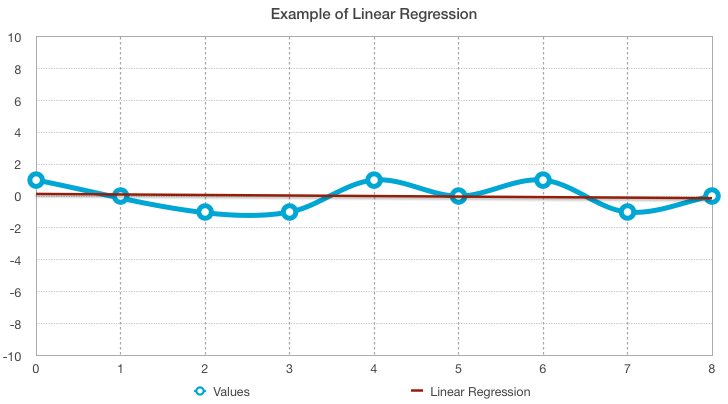
\includegraphics[width=100mm]{degree0.png}
\caption{Example of Linear regression}
\label{fig:degree0}
\end{figure}

Linear regression is polynomial regression of degree 1, and generally takes the form

\begin{equation} \label{eq:polynomialFormSmall}
f(x) = c_0 + c_1 * x
\end{equation}

where \emph{$c_0$} is the y-intercept and \emph{$c_1$} being the slope. Figure \ref{fig:degree1} shows clearly that the linear regression line running along the data points approximate the data. Mean average and linear regression are the most commom forms of polynomial regression, but not the only.

\begin{figure}[ht!]
\centering
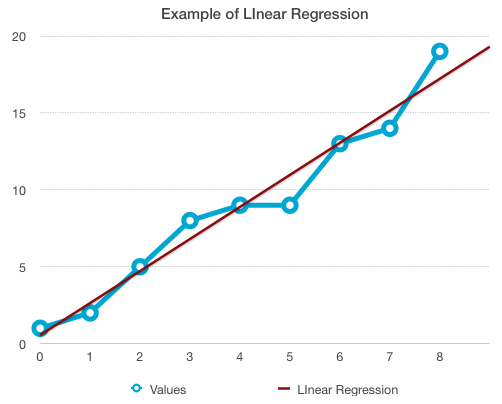
\includegraphics[width=100mm]{degree1.png}
\caption{Example of Linear regression}
\label{fig:degree1}
\end{figure}

The next step of polynomial would be the quadratic regression, now the regression becomes non-linear and the data is not restricted to straight lines. With figure \ref{fig:degree2} is possible to visualize a data with a quadratic regression trend line. Basically, the idea is simple: find a line that best fits 
the data which is find the coefficients to a polynomial that best fits the data.

\begin{figure}[ht!]
\centering
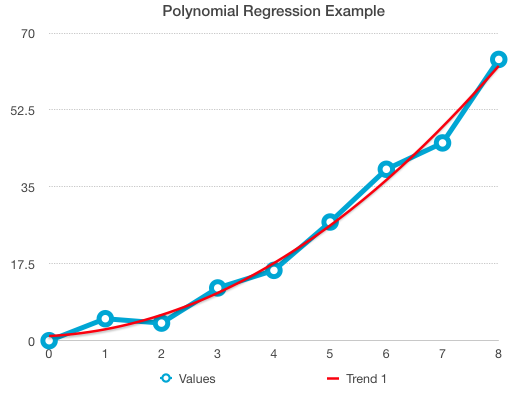
\includegraphics[width=100mm]{degree2.png}
\caption{Example of Polynomial Regression}
\label{fig:degree2}
\end{figure}

Polynomial regression is an overdetermined system of equations that uses least squares as a method of approximating an answer. To understand this, some linear algebra is required. 


%ACTIVITY OF A SOLUTE
\subsubsection{Activity of a solute}
Activity (\ce{a_i}) is \emph{"thermodynamic concentration"} (or informally known as \emph{"effective concentration"}). It is calculated as a product of activity coefficient and concentration (where \emph{i} means the solute involved):
\begin{equation}\label{activityEq}
a_i = \gamma_i * m_i
\end{equation}
Activity coefficient ($\gamma_i$) is a function of ionic strenght (I), which is a measure of the concentration of ions in the solution.  

%IONIC STRENGTH
\subsubsection{Ionic strength}
Mathematically the ionic strength of the solution is calculated according to
\begin{equation} \label{eq:ionicStrength}
I = 0.5 \sum{M_i z_i^2}
\end{equation}
where \emph{M} is the molar concentration of the specie \emph{i} having a charge \emph{z}.When \emph{I} increases, activity coefficients decrease. In very diluted solutions activity coefficient is equals to \emph{1.0} and activity is equal to concentration. The decreasing trend is related to the "cage" of opposite charge particles around ions. There is reversal of the trend in extremely concentrated solutions (brines) because beyond ionic strenght of about $1 mol/L$ there is an increase of activity coefficients with increasing ionic strength. This is related to decreasing amount of free water because most of water is already bound around dissolved species.
For a matter of explanation, we will calculate the ionic strength of a \ce{CaCl_2} solution (composed by $0.5 mol$ of \ce{Ca^{+2}} and $1 mol$ \ce{Cl^{-1}}):
\begin{eqnarray}
I = \frac{1}{2}  (z^2_{Ca}[Ca^{+2}]) + \frac{1}{2}  (z^2_{Cl}[Cl^{-1}]) \\
I = \frac{1}{2}  (2^2_{Ca}[Ca^{+2}] +  (-1)^2_{Cl}[Cl^{-1}]) \\
I = \frac{1}{2} (4 * 0.5 + 1 * 1) \\
I = 1.5 mol/L
\end{eqnarray}


%ACTIVITY COEFFICIENT
\subsubsection{Activity Coefficient} 
There are different methods to calculate $\gamma$ for ions:
\begin{itemize}
\item Debie-Hueckel: They assumed that ions behave like spheres with charges located at their center points. The ions interact with each other by coulombic forces and the result of their analysis is as follows
\begin{eqnarray} \label{eq:debyeEq}
log \gamma_i &=& - Az_i^2\sqrt{I}
\end{eqnarray} 
where \emph{A} is a constant that is a function of temperature, \emph{$z_i$} is the ion charge and \emph{I} is the ionic strength of the solution.
\item Davies equations: Is a variation of Debie-Hueckel that can be used when the ionic strength is relatively high. The equation is as follow
\begin{eqnarray} \label{eq:daviesEq}
log \gamma_i &=& - Az_i^2 \bigg(\frac{\sqrt{I}}{1+\sqrt{I}} - 0.3 I)
\end{eqnarray}
\item B-dot: This model is presented as an activity model based on an equation similar to Davies and parameterized for solutions up to 3 molal ionic strength.
\begin{eqnarray} \label{eq:bdotEq}
log \gamma_i &=& - \frac{Az_i^2 \sqrt{I}}{1+ a_i B \sqrt{I}} + \overset{.}{B} I )
\end{eqnarray}
where \emph{\aa}  is the ion size for each specie and \emph{A, B and $\overset{.}{B}$} are coefficients that vary with the temperature.
\end{itemize}
Important to mention that there are other methods available to calculate activity coefficients which are not going to be addressed here. Is important to keep in mind that pure solids have an activity equals to one.
Each one of the methods has its advantages and limitations. Debye-Hueckel equations are simple to apply and extensible to include new species in the solution due to the fact that it requires a low number of arguments and specific arguments. Besides, Debye-Hueckel can be applied to the most important temperatures in the field of aqueous geochemist. Important to keep in mind that it works poorly when regarding moderate or high ionic strength.
Regarding dissolution and precipitation there is clearly a reaction happening during these processes, which means that some reactions are not in equilibrium. 

%SATURATION INDEX
\subsubsection{Saturation Index}
The saturation index (\emph{SI}) indicates the degree of saturation with respect to a given mineral, in other words, it defines if a reaction will be in equilibrium or not. \emph{SI} is expressed as
\begin{eqnarray} \label{eq:siEq}
SI &=& log (IAP / K )
\end{eqnarray}
when a mineral is in equilibrium with a solution the \emph{SI} is zero, a negative \emph{SI} indicates undersaturation and a positive \emph{SI} supersaturation. 
Ion Activity Product (\emph{IAP}) is calculated according to
\begin{eqnarray}
IAP &=& \frac{[C]^c [D]^d}{[A]^a[B]^b}
\end{eqnarray}
where [A], [B], [C] and [D] are activitys of each ion. The interpretation of \emph{IAP} is the following:
\begin{itemize}
\item IAP > K : The reaction is progressing from right to left, producing more products. In a ground water solution, the water is supersaturated.
\item IAP = K : The reaction is in equilibrium, there is no flow neither to the right nor to the left. In a ground water solution, the water and the mineral are in equilibrium.
\item IAP < K : The reaction is progressim from left to right, producing more reactants. In a ground water solution, the water is undersaturated.
\end{itemize}

With the \emph{SI} approach is possible to predict the reactive mineralogy of the subsurface from the groundwater data without collecting samples of the solid phase and analyzing the mineralogy. If the \emph{SI} for a mineral calculates to be less than zero, the aqueous solutions is undersaturated with respect to that mineral - which corresponds to the fact that the mineral will not precipitate and may dissolve in order to reach equilibrium concentrations. If the \emph{SI} is greater than zero, then the mineral is not reactive and the mineral may precipitate from the aqueous solution (oversaturated). To conclude, when the \emph{SI} is close to zero (it is ok to consider a small range of values to be in equilibrium) , it means that the water is saturated  with respect to that mineral \cite{Alley:93}. From the mentioned before, it is possible to state the following:
\begin{itemize}
\item SI < 0 : Mineral is undersaturated;
\item SI = 0 : Mineral is in equilibrium with the solution;
\item SI > 0 : Mineral is oversaturated;
\end{itemize}

%HYDROGEOCHEMISTRY COMMON UNITS
\subsubsection{Hydrogeochemistry common units}
Molarity (\emph{M}), defined as mass in moles in 1 liter of solution and molality (\emph{m}), defined as mass in moles in 1 kilogram of solution. In dilute solution molarity is approximately equal to molality. Concentration in miliequivalents per liter is concentration in milimoles per liter multiplied by charge of an ion.

%HYDROCHEMICAL PROCESSES
\subsection{Hydrochemical processes}

%ACID-BASE REACTIONS
\subsubsection{Acid-Base Reactions}
The importance of acid-base reactions is cleary when it is understood its influence on the pH. The pH is a master variable in charge of controlling chemical systems and is described as
\begin{eqnarray}
pH = - log([H^+])
\end{eqnarray}
where $[H^+]$ is the activity of the hydrogen ion. The interpretation of the values is as follows:
\begin{itemize}
\item pH < 7 : acid solution;
\item pH = 7 : neutral solution;
\item pH > 7 : basic solution;
\end{itemize}
The acid substance has tendecy to lose protons while a base substance has tendency to gain protons and the interation between acids and bases is called acid-base reactions and is described as
\begin{eqnarray}
Acid_1 + Base_2 &=& Acid_2 + Base_1
\end{eqnarray}
The reaction must be understood as that in the forward reaction, the proton lost by $Acid_1$ is gained by $Base_2$ and in the reverse reaction the proton lost by $Acid_2$ is gained by $Base_1$.  The strength of an acid or base refers to the proportion of its protons are lost or gained. 

%COMPLEXATION AND SPECIATION
\subsubsection{Complexation and Speciation}
A complexation is when an ion that forms by combining simpler cations, anions and sometimes molecules, this process facilitates the transport of potentially toxic substances and form what is called a complex. Due to the importance of this process in contamination problems it has acquired a huge importance in practical and commercial fields. A simple example of complexation is the following
\begin{eqnarray}\label{complexation_reaction}
Mn^{2+} + Cl^- &=& MnCl^+
\end{eqnarray}
Calculation of distribution of metals mong complexes (\emph{speciation}) involves the solution of a series of mass-law transport equations. The mass law equation of the reaction ~\ref{complexation_reaction} is described bellow
\begin{eqnarray}
K_{MnCl^+} &=& \frac{[MnCl^+]}{[Mn^{2+}][Cl^-]}
\end{eqnarray}
Each one of the complex has a variable associated called stability constant ($\beta_i$)  and it contains the basic information necessary to determine how the total concentration of a metal in a solution is distributed as a metal ion and the other various complexes possible. 

%OXIDATION-REDUCTION REACTIONS
\subsubsection{Oxidation-Reduction Reactions}
Groundwater environemnt's reactions involve transfer of electrons between its components (gaseous, dissolved or solid constituents). As result, there are changes in the oxidation states of the reactants and products. It is important to stress that the oxidation number is a hypothetical charge that an atom would have if the ion or molecule were to dissociate. This state can be different according to the solution. 
During this work, \emph{redox reactions} (as oxidation-reduction reactions are also known) are not going to be addressed. In order to get deeper understanding on this topic, we refer to \cite{Petrucci:07}

%ADSORPTION AND ION EXCHANGE
\subsubsection{Adsorption and ion exchange}
Adsorption systems treat water by adding a substance, such as activated carbon or aluminia, to the water supply. Adsorbents attract contaminants by chemical and physical processes that cause them to \emph{stick} to their surfaces for later disposal. This mechanism is often used to remove contaminants like \emph{arsenic} or \emph{fluoride} (mostly organic contaminants) from water reservoir.
Ion exchange work simillarly but it is focused in inorganic contaminants in a particle-free water. Ion exchange is most often used to remove hardness or nitrate (mostly inorganic soluble molecules). 
During this work, adsorption and ion exchange are not going to be addressed. In order to get deeper understanding on this topic, we refer to \cite{Freeze:79}

% GEOCHEMICAL MODELLING
\subsection{Geochemical Modelling}
The geochemical modelling is the design of the geochemical reactions responsible for the migration of dissolved species. Geochemical models can be divided into two groups:
\begin{itemize}
\item Geochemical Equilibrium Models: Based on the assumption of thermodynamic equilibrium reached in a relatively short time (no time factor is included in calculation). It takes in consideration only equilibrium reactions.
\item Geochemical Kinetic Models: It takes into account also kinetic reactions and includes the time factor. As kinetic data is measured experimentally, there is still a lack of kinetic data available for many geochemical processes. 
\end{itemize}

As mentioned before, this work will focus on the first one - \emph{geochemical equilibrium models}.

Inside geochemical equilibrium models we can mention three divisions: speciation models; inverse models (also called mass balance models); forward models (also called reaction path models); and reactive transport (coupled) models. Regarding the relation to spatial coordinates, geochemical equilibrium models are considered \emph{batch models} - which are basically closed vessels or reactors.

%GEOCHEMICAL SPECIATION MODELLING
\subsubsection{Geochemical Speciation Modelling}
Speciation represents modelling based in the equilibrium of the system. A geochemical speciation modelling program calculates the distribution of dissolved species between free ions and aqueous complexes and also saturation indexes for different minerals. Sodium, for example, can be present in water as free ion \ce{Na^+}, and also in the form of complexes with anions:

\begin{equation}
\ce{Na^+}_{total} = \ce{NaCl}_{aq} + \ce{NaOH} + \ce{Na^+}
\end{equation}

where \ce{Na^+_{total}} is total sodium concentration from chemical analysis. \ce{Na^+_{total}} is a component (e.g., chemical formula unit used to describe a system) and \ce{Na^+}, \ce{NaCl_{aq}} and \ce{NaOH} are species (chemical entities which really exist in the system). Information about the distribution of dissolved species is important, for example, for risk assessment of contamination by metals because toxicity of metails depends on their speciation in solution. Carbonate complexes of metails, for example, are less toxic than their free ions.
Saturadio index (SI) is used to determine the direction of geochemical processes. When \emph{SI > 0} the mineral precipitates from the water and when \emph{SI < 0}, the mineral dissolves in contact with the water, if it is present in solid phase. Field data necessary for input of speciation program are temperature, pH and results of laboratory chemical analysis (results from a sampling of the solution of interest).

Common problems solved using speciation programs are: 
\begin{itemize}
\item There is a sample with high concentration of dissolved sodium and we need to know the distribution of sodium between \ce{Na^+} and different complexes (for example, \ce{{NaCl}_{aq}} or \ce{NaOH}) because different forms of sodium have different characteristics;
\item There are ground water samples that had been in contact with granitic masses and we want to verify the possibility of precipitation of minerals like \emph{Albite} (a plagioclase feldspar mineral whose formula is \emph{\ce{NaAlSi_{3}O_{8}}}).
\end{itemize}
Note that the details of several available programs are going to be presented and discussed in chapter ~\ref{chapter:review}).

The development of our software \emph{SHPECK}, which is a geochemical speciation modelling software will be detailed, presented and thoroughly discussed in chapter~\ref{chapter:SHPECK}. Also important to mention that this work is the first work that will completely guide anyone to generate a geochemical speciation modelling software from the ground.

%OTHER TYPES OF GEOCHEMICAL MODELLING
\subsubsection{Other Types Of Geochemical Modelling}
\begin{itemize}
%INVERSE GEOCHEMICAL MODELLING
\item Inverse geochemical modelling
This type of models, also known as mass balance models, are used when chemistry of groundwater and solid phase composition are already known, and reactions that have already happened should be determined. It is used when we have access to 2 hydraulically connected points and composition of solid phase between these points; with these data in hand, it is possible to calculate and produce the reactions that will explain the changes of the water's chemistry. This approach leads to some uncertainties: Stoichiometry of minerals in solid phase is not often well known; solution may be non-unique; and programs can produce several possible models for the same input;
An interesting work about inverse geochemical modelling can be verified in \cite{Sharif:07}.
%FORWARD GEOCHEMICAL MODELLING
\item Forward geochemical modelling
This type of models, also called reaction path models, are used for prediction of water chemistry evolution along a flowline. Initial water chemistry is known and the aim of the program is to predict water chemistry at some point along flow path. This kind of modelling introduce problems regarding kinetic and adsorption data, which are ofter missing and frequently limited. 
\end{itemize}

\newpage

%SUMMARY
\section{Summary}
\begin{itemize}
\item Importance of multidisciplinary problems: The amazing power of computer science to adapt itself to other areas of knowledge and do something brilliant is incredible. The best way to push the limits is by redefining obstacles outside normal boundaries and reach solutions based on new understanding of complex situations.
\item Computer science principles: Understanding what is a software and how it connects with the \emph{"machine world"} to the \emph{"real world"} is something not trivial. We reinforce the idea that the extension of a software goes way beyond the lines of code and the interface showing up on the screen.We often find the comparison that building software is somehow like building a house - this certainly is a helpful example to understand everything that is behind a software. Both house and software require: estimating costs, thinking about the requirements, plans, rules, standards, best practices, specifications timelines, reviews, milestones, testing, alterations, handover and warranty.
\item Hydrogeochemistry principles: Thermodynamics is one of the substantial basis for the history of physics, chemistry and the science in general as we know it. It is crucial to understanding the role that it has in the natural aspects of the world that we live. The comprehension of thermodynamics goes through the analysis, awareness and interrelations of the several factors that compose this complex \emph{maze}. From the wide range of factors, we can mention the equilibrium and kinetic reactions, the activity and the activity coefficient of the solute, the ionic strength of the solution, the saturation index, etc.
\end{itemize}


%%%%%%%%%%%%%%%%%%%%%%
%                                                                 %
% COMMERCIAL SOFTWARES REVIEW  %
%                                                                 %
%%%%%%%%%%%%%%%%%%%%%%

%COMMERCIAL SOFTWARES REVIEW
\chapter{Commercial softwares review}
\label{chapter:review}
The importance of geochemical models has increased lately due to its variety of applications, but the first models date back to the 70’s as in \cite{Westall:76} and \cite{Wolery:79}. Since then, these models are used to solve problems as  speciation; determination of minerals' saturation indexes; adjustment of equilibrium for minerals; mixing of different waters; calculation of stoichiometric reactions; mixing of solids, fluids and gaseous phases; calculation of equilibrium/kinetic controlled reactions; reactive transport; mass-law calculations;

The quality of the chemical analysis depend on the methods used, thermodynamic data and theoretical concepts applied. Therefore it is crutial to check the results and is clear that there will be some differences in the results according to the software used. Among the huge variety of software availables, some of them are developed for batch-type simulations only while others have transport capabilities. Several of them do not incorporate graphical interfaces and are written in FORTRAN, newer distributions are mainly written in C/C++ and due to proprietary reasons code is not distributed along the software. Important to mention that, even those who have an integrated graphical user interface (GUI), it is ofter very tedious and time-consuming to generate input files for groudwater simulation softwares.

The goal of this chapter is to note other codes that perform modelling of aqueous geochemical systems. It is not possible nor the purpose of this work to present all the existing codes but to critically review and compare some aspects of the codes. These codes are being widely used among the community and have enough documentation published in the open literature that makes a comparison effort sustainable and interesting.

During this work we will focus exclusively on programs that do specifically speciation models. Which are the following: \emph{EQ3/6}; \emph{PHREEQC}; \emph{MINTEQ}; and \emph{SOLMINEQ};

We will present each relevant detail about the geochemical point of view and then  critically analyze and discuss from the computer science point of view. It's worth mentioning that in any aspect this review is meant to be impolite. Quite the opposite, we value their efforts and are thankful by the knowledge we could acquired by using and analyzing them. We ask the reader's comprehension in order to understand that sometimes is not possible to analyse the same aspects of different softwares due to the lack of information available. 


%GEOCHEMICAL SPECIATION MODELLING CODES
\section{Geochemical Speciation Modelling Codes}

%EQ3/6
\subsection{\emph{EQ3/6}}
EQ3/6 consists of two programs: EQ 3 is a pure speciation code whose results EQ 6 subsequentially process. It is a software package for geochemical modeling of aqueous systems written in FORTRAN77. EQ3/6 includes a speciation-solubility solver (useful for analyzing groundwater chemistry data, calculating solubility limits and determining whether certain reactions are in states of partial equilibrium or disequilibrium). It also offers a reaction path calculation that models water/rock interaction or fluid mixture. EQ3/6 supports several thermodynamic data files (these data files contain support for Davies, B-dot, Debye-Hueckel equations, as well as support data for standard state and activity coefficient-related). It is developed to run under UNIX, and the distribution is not free (it requires a license). \cite{Wolery:79} \cite{Wolery:90} \cite{Wolery:92}.

\subsubsection{User Interactions}
In \emph{EQ3/6} the command prompt is responsible for all the interactions with the user. There are several codes inside \emph{EQ3/6} and each one of them must be run with the appropriate command prompt shortcut. From the existing softwares there are \emph{EQ3NR}, \emph{EQ6} and \emph{EQPT} just to name a few.The user must enter command from the keyboard and must use this "command prompt". By pressing "CTRL+C" at any time the software execution stops, literally "breaking" the process. For example, EQ3 is run by commands of the form as in code ~\ref{eq3:run}.

\begin{lstlisting}[frame=single, caption=Running EQ3 in \emph{EQ3/6} package, label=eq3:run]
>runeq3 datafilekey inputfile(s)
\end{lstlisting}

Where \emph{datafilekey} and \emph{inputfile} are arguments used by the program; The former is a three-character identification associated to which database should be used while the latter is specifically the name of the input file (can be more than one). Depending on which program from the package the user is using, two to several output files are going to be generated, always in the \emph{ASCII} format. 
As mentioned, the inputfile will be entered in the program as an argument. Any regular text editor is sufficient to create or modify an input file (although it is strongly recommended that the user does not create an input file from scratch). There are several pre-existing input templates available and if none of them matches the need of the user, \emph{EQ3/6} recommends that the user generate a new one by copying existing blocks from these templated provided.

The menu format inside the input files try to recriate known user interactions method as shown in code ~\ref{eq3:menu}.

\begin{lstlisting}[frame=single, caption=Menu Option inside \emph{EQ3/6} input files that mimics a "radio button", label=eq3:menu]
iopr(4) - Print a Table of Aqueous Species Concentrations, Activities, etc.: 
 [ ] (-3) Omit species with molalities < 1.e-8 
 [ ] (-2) Omit species with molalities < 1.e-12 
 [ ] (-1) Omit species with molalities < 1.e-20 
 [x] ( 0) Omit species with molalities < 1.e-100 
 [ ] ( 1) Include all species 
\end{lstlisting}

\subsubsection{Input/Output Options}
The \emph{datafilekey} and \emph{inputfile} given to the program as arguments must be consistent with the options and methods. For example, if they have different mehtods for calculating the activity coefficient there will be problems and the results will be meaningless. Other point to be taken into consideration and that follows the same idea, the \emph{inputfile} must be using chemical data (for example, elements, species and compounds) that is known by the \emph{datafilekey}. 

Inside each file, there are a series of \emph{blocks} that combined together in order to do the geochemical speciation. They are presented bellow:
\begin{itemize}
\item \emph{Datafilekey}: Title; Miscellaneous parameters (temperature limit, activity coefficient parameters, pressure); Chemical elements block; Aqueous species block; Pure minerals block; Pure non-aqueous liquids block; gas species blocks; solid solutions blocks; references blocks;
\item \emph{Inputfile}: Title; Special basis switches; temperature; pressure option; density; total dissolved salts (TDS) option; electrical balancing option; redox option; basis species constraints; ion exchanger creation flag; ion exchanger compositions; solid solutions compositions; alter/suppression options; iopt options; iopg options; iopr options; iodb options; numerical parameters; ordinary basis switches; saturation flag tolerance; aqueous phase scale factor;
\end{itemize}

EQ3/6 package produces different output depending on the software that is used. We will exemplify the output files in general by using the \emph{EQ3NR} and \emph{EQ6} output formats. 
\begin{itemize}
\item \emph{EQ3NR}: There will be generate two output files. A \emph{pickup} file and the normal output file. The \emph{pickup} file can be used as input to \emph{EQ6} software. The normal output file consists of six \emph{blocks}: header secion; input file echo; recap of input data; iterative calculations; principal results; and finally the end of EQ3NR run;
\item \emph{EQ6}: There will be generated three output files. An \emph{tab} output file, a \emph{pickup} output file and the normal output file. The \emph{tab} file contains information that can be used to plot output results. The \emph{pickup} file can be used as input to \emph{EQ6}. The normal output file consists of six \emph{blocks}: header; input echo; input recap; iterative calculations; principal results; and finally the end of \emph{EQ6} run; 
\end{itemize}

A small excerpt of an \emph{EQ6} outpuf file is shown in code ~\ref{eq3:output}.

\begin{lstlisting}[frame=single, caption=Excerpt of \emph{EQ6} output file, label=eq3:output]
...
 Entity Date Base Dimension Current Problem
 Chemical Elements 81 81 6
 Basis Species 201 259 7
 Phases 1135 1159 29
 Species 3031 3523 0
 Aqueous Species 1769 1769 22
 Pure Minerals 1120 1120 26
 Pure Liquids 1 3 1
 Gas Species 93 93 2
 Solid Soutions 12 12 0
...
\end{lstlisting}


\subsubsection{File Formats}

All the files discussed above are in the \emph{ASCII} text files format and, therefore, any regular text editor is able to be used. When the text file is a database, it is converted to binary format and this binary will be used directly by the softwares. This conversion from text files (\emph{ASCII}) to binary file is somehow interesting. An \emph{ASCII} file is a binary file that consists of \emph{ASCII} characters. \emph{ASCII} characters are 7-bit encodings stored in a byte. Thus, each byte of an \emph{ASCII} file has its most significant bit set to 0 which leads to waste of a bit for every byte - propagate this to a significant amount of \emph{ASCII} information and it is possible to understand the reason for this conversion. Another reasonable advantage for the binary files is that the search in binary files is normally faster than in \emph{ASCII} files.

\subsubsection{Software Environment}
The \emph{EQ3/6} package runs in Windows (95 and upper versions). The support for UNIX computers has been discontinued.  It is written in FORTRAN77 and has been eveloped and run at Lawrence Livermore National Laboratory on an Alliant FX/80 and Sun SPARCstations. 
\subsubsection{Installation Procedures}
The installation of \emph{EQ3/6} is explained in details in \cite{Wolery:92}. Due to the purpose of this work, details of the installation will be supressed here. At the same time, it is interesting to mention that the whole installation process is also done through the command prompt and requires some level of experience. 

%PHREEQC
\subsection{\emph{PHREEQC}}
\emph{PHREEQC} stands for \emph{PH} \emph{RE}dox \emph{EQ}uilibrium (in \emph{C} language) and is a widely used public-domain geochemical modelling software available from the USGS. It is available to download for free with versions for PC and Mac. Designed to perform a wide variety of low-temperature aqueous geochemical calculations based on an ion-association aqueous model and has capabilities to:
\begin{itemize}
\item Speciation and Saturation Index calculations;
\item Batch reaction and one-dimensional (1D) transport calculations involving reversible reactions (including aqueous, minerals, gas, solid-solution, surface-complexation, and ion-exchange equilibrium) and irreversible reactions (including specified mole transfer of reactants, kinetically controlled reactions, mixing of solutions and temperature changes);
\item Inverse modelling, which finds sets of mineral and gas mole transfers that takes into account differences in composition between waters.
\end{itemize}
The software was written in C and has free distributions for Windows, Linux and MAC \cite{Parkhurst:80}.

\subsubsection{User Interactions}
\emph{PHREEQC}'s distribution differs drastically according to the environment (\emph{Windows} or \emph{UNIX}). By this reason, the analysis of user interactions will be done separately.
\begin{itemize}
\item \emph{PHREEQC} for Windows: Due to the need of a geochemical modelling software and the lack of interface for \emph{PHREEQC} on the first versions of the software, many efforts were done in order to create a interface to \emph{PHREEQC}. The program \emph{PhreeqcI} is a graphical user interface to \emph{PHREEQC} that provides data entry screens for the keyword data blocks with a description of each input data item. Organizing the input file by using some sort of \emph{project tree} which facilitates viewing, selecting, editing and running the \emph{PHREEQC} simulations. Very important to mention that some keyword blocks are not implemented on \emph{PhreeqcI}. After this, another effort was done, \emph{PHREEQC} version 2 was launched with a graphical interface - which was kept later in version 3. The last effort in this sense was the development of an adaptation of the popular general-purpose text editor \emph{Notepad++}. This mod comes with the following capabilities: syntax highlighting; autocompletion of keywords and identifiers; tips; colored numbers; parenthesis matching; commenting and uncommenting multiple lines at once; column editor; few shortcuts; and file recognition;
\item \emph{PHREEQC} for UNIX: Under UNIX's distribution, \emph{PHREEQC} runs from the command prompt. It can be used by using the command as in code ~\ref{phreeqc:run}
\begin{lstlisting}[frame=single, caption=Command to run UNIX's \emph{PHREEQC}, label=phreeqc:run]
phreeqc input output database screen_output
\end{lstlisting}
Where \emph{"input"} file will contain the description of the simulation, the \emph{"output"} file will store the results of the simulation, \emph{"database"} will specify which database should be used and \emph{"screen\_output"} stores the information that will be shown on screen. If the user doesn't specify the names of \emph{"output"}, \emph{"database"} or \emph{"screen\_output"} the geochemical modelling software will choose default values.

\end{itemize}
\subsubsection{Input/Output Options}
The input data for \emph{PHREEQC} is arranged by \emph{keyword data blocks}. Each block organized with a keywork on the first line followed by lines containing data related to the keyword. Keywords and its context are read from the database at the beginning of the run to define all the necessary parameters - interesting to keep in mind that \emph{any} parameters can be redefined on the input file if the user wants. After the database is read, it will continue reading the input file until the \emph{END} keyword is reached. This process will be repeated until the end of the file. As the input file is being read, the program will start putting the pieces together in order to perform the necessary calculations. An example of a \emph{keyword data block} is shown in code ~\ref{phreeqc:keyword}. Among the possible keywords available in \emph{PHREEQC} are: EQUILIBRIUM PHASES, EXCHANGE, GAS PHASE, INVERSE MODELING, PHASES, REACTION, PRINT, SAVE, SOLUTION SPECIES, etc. Each one of these keywords contains specific arguments and parameters in order to be used. Certain keywords require some specific others keywords - somehow like a puzzle - and if there is something missing on the input file, the results are going to be inconclusive and wrong.

\begin{lstlisting}[frame=single, caption=\emph{PHREEQC} keyword data block example, label=phreeqc:keyword]
EQUILIBRIUM_PHASES
Chalcedony  0.0     0.0
CO2(g)      -3.5    1.0
Gibbsite(c) 0.0     KAlSiO8  1.0
Calcite     1.0     Gypsum   1.0
pH_Fix      -5.0    HCl      10.0
\end{lstlisting}


The output file will contain the results of the simulation defined on the input file also divided in \emph{keyword blocks}. Among those we can mention solution composition, description of solution, redox couples, distribution of species (as can be seen in code ~\ref{phreeqc:output}), saturation indices.

\begin{lstlisting}[frame=single, caption=\emph{PHREEQC}'s excerpt from the output file, label=phreeqc:output]
...
----------------------------Distribution of species----------------------------
 
                                               Log       Log       Log    mole V
   Species          Molality    Activity  Molality  Activity     Gamma   cm3/mol
 
   OH-            2.705e-006  1.647e-006    -5.568    -5.783    -0.215     -2.63
   H+             7.983e-009  6.026e-009    -8.098    -8.220    -0.122      0.00
   H2O            5.551e+001  9.806e-001     1.744    -0.009     0.000     18.07
C(4)         2.257e-003
   HCO3-          1.238e-003  8.359e-004    -2.907    -3.078    -0.170     27.87
   NaHCO3         6.168e-004  7.205e-004    -3.210    -3.142     0.067     19.41
   MgHCO3+        2.136e-004  1.343e-004    -3.670    -3.872    -0.201      5.82
   MgCO3          7.301e-005  8.527e-005    -4.137    -4.069     0.067    -17.09
   CaHCO3+        3.717e-005  2.572e-005    -4.430    -4.590    -0.160      9.96
   CO3-2          3.128e-005  6.506e-006    -4.505    -5.187    -0.682     -0.34
   CaCO3          2.256e-005  2.636e-005    -4.647    -4.579     0.067    -14.60
   NaCO3-         1.477e-005  9.972e-006    -4.831    -5.001    -0.170      1.77
   ...
\end{lstlisting}

\subsubsection{File formats}
All the files discussed above are in the \emph{ASCII} text files format and, therefore, any regular text editor is able to be used. It is recommended that the edition of the \emph{PHREEQC} files is done by using its own interface.

\subsubsection{Software Environment}
\emph{PHREEQC} has support for Windows (32 and 64-bit), MacOS (OS 10.6+) and Linux. \emph{PHREEQC} is currently on version 3 and the frequency of updates, bug fixes and maintenance is fine.

\subsubsection{Installation Procedures}
The \emph{PHREEQC} version for Windows has a self-extracting file that can be downloaded from the USGS website and easily installed. The \emph{UNIX} distribution comes with additional scripts and a makefile and the user should follow some steps to compile and install the program.


%MINTEQ
\subsection{\emph{MINTEQ}}
Much simpler options on raction treatment, developed by the United States' Environment Protection Agency (EPA). 

Is an equilibrium speciation model that is used to calculate equilibrium composition of dillute aqueous solutions. The model is useful for calculating the equilibrium mass distribution among disolved species, adsorbed species and multiple solid phases. A large database adequate to a large range of problems is inclued and there is no need for the user to change or add anything \cite{Brown:87} \cite{Allison:91}.

\subsubsection{User Interactions}
\subsubsection{Input/Output Options}
\subsubsection{File formats}
\subsubsection{Software Environment}
\subsubsection{Installation Procedures}

\subsection{\emph{SOLMINEQ}} "ITS A DATABASE FOCUSED IN ORGANIC MATERIAL"
Is a FORTAN 77 written geochemical modeling program based on SOLMNEQ with improved algorithms that result in a faster program execution and tighter convergence. Has a database with over 270 inorganics and 80 organics aquoues species and 214 minerals. It calculates the distribution of mass among aquoues species and complexes and calculates saturation indexes of minerals at different temperatures and pressures. It includes a wide variety of options, for example, boiling, mixing of solutions and partitioning of gases between water, oil and a vapour phase. Solimineq.88 contemplates also mass trasnfer with the effects of dissolution and/or precipitation of minerals and options to calculate activity coefficient model. The original version has no GUI but there were further studies with the intention of creating a user-friendly program that can be used to edit/analize input and output files of Solmineq.88 \cite{Kharaka:73}.

\subsubsection{User Interactions}
\subsubsection{Input/Output Options}
\subsubsection{File formats}
\subsubsection{Software Environment}
\subsubsection{Installation Procedures}

\section{Summary}

%GEOCHEMICAL SPECIATION ANALYSIS
\section{Geochemical Speciation Analysis}
The idea is to do a table comparison of softwares and tech details. Also interesting to mention who maintain (OR NOT) the programs.

%SHPECK ANALYSIS
\section{SHPECK Analysis}

%SUMMARY
\section{Summary}


%%%%%%%%%%%%%%%%%%%
%                                                        %
% SHPECK - SPECIATION MODEL  %
%                                                        %
%%%%%%%%%%%%%%%%%%%

\chapter{\emph{SHPECK} - Speciation Model}
\label{chapter:SHPECK}
\begin{itemize}
\item	Global vision of a simulator
\item	Architecture of a simulator
\item	Mathematical treatment and details
\item	Technologies being used
\item	Software engineering
\item	Program organization
\item	Complexity of the algorithm

Calculation of speciation is conducted by substitution of the equilibrium constants into the mass balance expressions for the total concentration of a particular component. This results in a series of nonlinear equations which are solved iteratively using numerical techniques, such as the Newton-Raphson iteration used in the MINTEQA2 model. Iterations continue until the total calculated component concentrations, derived from the equilibrium expressions, calculated activity coefficients, and component mass balances, and the measured total concentrations converge to a prescribed limit [Nordstrom, 1979 #3004].

\item	Data-flow
\item	User interface description and details
\item	Database: criterios de comparacao do pq usar um banco de dados estruturado; comparacao de tempo com o arquivo texto; simular pesquisa com os 2 formatos; consulatas elaboradas; concatenacao de elementos com queries; espaco, tempo e expressividade; uso de BD em area nao difundida.
\item	Summary
\end{itemize}

%%%%%%%%%%%%%%%%%%%%%%%%
%                                                                       %
% CASE STUDY, RESULTS, COMPARISON   %
%                                                                        %
%%%%%%%%%%%%%%%%%%%%%%%%%

\chapter{Case Study, Results and Comparison}
\begin{itemize}
\item Explanation of the data that will be used to compare the results: 
\item Results comparison 
\item	Summary
\end{itemize}

Results from initial studies indicated that the uncertainty for thermodynamic values is much greater around the very dilute range and the more concentrated range, where data for the thermodynamic constants are comparatively sparse. 

%%%%%%%%%%%
%                            %
% CONCLUSION   %
%                            %
%%%%%%%%%%%

\chapter{Conclusion}

Geochemical speciation is critical for understanding the form of chemicals of interest in natural systems. It is crucial in many different aspects of our daily life nowadays: assessing bioavailability, risk to humans and ecosystems. Geochemical speciation models are generaly determined through analytical methods that measure free ions or total concentrations, used in conjunction with thermodynamically based models. As presented on this work, these models rely on the local equilibrium assumption, and on experimentally determined reaction constants. It is clear, though, that if the chemical system does not achieve equilibrium state or if the equilibrium constants are not certain, the geochemical speciation model's prediction show significant uncertainty.
This emphasizes the clear need for a proper computation approach while treating with such influential information like a geochemical speciation model. The information flow is tightly connected and any mistake will propagate errors and carry that wrong information until the very end of the model.

\begin{itemize}
\item Review of the results emphasizing our approach and advantages
\item  Geological explanations for the results
\item  Final discussion about \emph{SHPECK}
\item  CONTRIBUTION (EXPLICIT AND WELL DESCRIBED) 
\end{itemize}


%This work provides three important steps of the development of a geochemical modeling speciation software with the purpose of increasing the quality in such field of softwares. The development of a new software is intended to raise and optimize in every possible way the concept of geochemical modelling always taking into account the computer science priorities and theory. The difference between all the options and this work's approach is that the computer science's side is taken more responsibly and strategically thought since the beginning. What have been notested from all existing softwares studied is that they were created by geochemists, chemicals, geologists to solve their daily challenge and questions - our approach is different: it is done by computer science specialists with the support of geologists and geochemicals. Naturally some challenges are faced, for example, the base concepts are sometimes misunderstood and it is mandatory that the basic concepts are well stablished in order to have a solid and useful software in the end of the process. During the process of developing this work aspects of physical chemistry, aqueous geochemistry, linear algebra, complex coupled systems and computational simulatosrs are going to be studied and learned.

% references



\makeglossaries

\renewcommand*\bibname{References}
\begin{thebibliography}{este-parametro-nao-eh-usado-pelo-estilo-ABNT}

\bibitem[GARRELS, 1965]{Garrels:65} R. M. GARRELS AND C. M. CHRIST
 \textbf{Solutions, Minerals, and Equilibria}: Harpers' Geoscience Series. Harper and Row, New York, 1965.

\bibitem[KEHEW, 2000]{Kehew:00} KEHEW, A.
 \textbf{Applied Chemical Hidrogeology}: Prentice Hall, 2000. 368p.

\bibitem[FREEZE, 1979]{Freeze:79} FREEZE, R. A. and CHERRY, J. A.
\textbf{Groundwater}: Prentice Hall 1979

\bibitem[DOMENICO, 1997] {Domenico:97} DOMENICO, P. A. and SCHWARTZ, F. W.
\textbf{Physical and Chemical Hydrogeology - Second Edition}: John Wiley and Sons Inc.

 \bibitem[DALE, 2004]{Dale:04} DALE, NELL B.
 \textbf{Programming and problem solving with C++}: Jones Bartlett Publishers, 2004.
   
\bibitem[WOLERY, 1979] {Wolery:79} WOLERY, T. J. 
\textbf{Calculation of chemical equilibrium between aqueous solution and minerals: \emph{the EQ3/6 software package}}: Lawrence Livermore National Laboratory, Livermore CA, U.S.A.

\bibitem[WOLERY, 1990] {Wolery:90} WOLERY, T. J., JACKSON, K. J., BOURCIER, W. L., BRUTON, C. J., VIANI, B. E., KNAUSS, K. G. and DELANY, J. M.
\textbf{Current status of the EQ3/6 software package for geochemical modeling in Chemical Modeling of Aqueous System}: ACS Symposium series, No 416, p 104-116. American Chemical Society, Washington, DC.

\bibitem[WOLERY, 1992] {Wolery:92} WOLERY, T. J.
\textbf{EQ3/6, a software package for geochemical modeling of aqueous systems: package overview and installation guide (Version 7.0)}: Lawrence Livermore National Laboratory, Livermore CA, U.S.A.

\bibitem[KHARAKA, 1973] {Kharaka:73} KHARAKA, Y. K. and BARNES, I.
\textbf{SOLMNEQ: Solution-Mineral Equilibrium Computations}: NTIS Tech Rept. PB214-899, Springfield, VA, 82p

\bibitem[NORDSTROM, 1986] {Nordstrom:86} NORDSTROM, D., MUNOZ, K.
\textbf{Geochemical Thermodynamics}: Prentice Hall, 200. 477p

\bibitem[PARKHURST, 1995] {Parkhurst:80} PARKHURST, D. L.
\textbf{User's guide to PHREEQC - A Computer program for speciation, reaction-path, advective-transport, and inverse geochemical calculations}: U.S. Geological Survey Water-Resources Investigations Report 95-4227, 143p

\bibitem[BROWN, 1987] {Brown:87} BROWN, D. S. and ALLISON, J. D.
\textbf{MINTEQA1, an equilibrium metal speciation model: user's manual}: Environmental Research Laboratory, Office of research and development, U.S. Environmental Protection Agency.

\bibitem[ALLISON, 1991] {Allison:91} ALLISON, J. D., Brown, D. S. and Novo-Gradac, K. J.
\textbf{MINTEQA2/PRODEFA2, a geochemical assessment model for environmental systems: version 3.0}: Environmental Research Laboratory, Office of research and development, U.S. Environmental Protection Agency.

\bibitem[Qt(2014)] {qt:14} Qt
\textbf{Application Framework}: Available at http://www.qt-project.org : Accessed in July 2014.

\bibitem[Armadillo(2014)] {arma:14} Arma
\textbf{Armadillo C++ linear algebra library}: Available at $http://www.arma.sourceforge.net$ : Accessed in July 2014.

\bibitem[LEE, 2011] {Lee:11} LEE, L. and GOLDHABER, M
\textbf{The Geochemist's Workbench Computer Program}: 

\bibitem[BETHKE, 1996] {Bethke:96} BETHKE, C. M.
\textbf{Geochemical Reaction Modeling, concepts and applications}: Oxford University Press, 397p

\bibitem[BETHKE, 2008] {Bethke:08} BETHKE, C. M.
\textbf{Geochemical and Biogeochemical Reaction Modeling}: Cambridge University Press, 547p

\bibitem[XU, 2004] {Xu:04} XU, T., SONNENTHAL, E.L., SPYCHER, N., PRUESS, K.
\textbf{TOUGHREACT User's guide: A Simulation program for non-isothermal multiphase reactive geochemical transport in variably saturated geologic media}: Lawrence Berkeley National Laboratory, Berkeley, California, U.S.

\bibitem[HARBAUGH, 2000] {Harbaugh:00} HARBAUGH, A. W., BANTA, E. R., MCDONALD, M. G.
\textbf{MODFLOW-2000, the U.S. Geological Survey modular ground-water model - User guide to modularization concepts and the Ground-Water Flow Process}: U.S. Geological Survey

\bibitem[NOFZIGER, 2000] {Nofziger:00} NOFZIGER, D. L., WU, J.
\textbf{CHEMFLO : Interactive software for simulating water and chemical movement in unsaturated soils}

\bibitem[PETRUCCI, 2007]{Petrucci:07} PETRUCCI, RALPH H.
\textbf{General Chemistry: Principles \& Modern Applications}: New Jersey : Prentice-Hall

\bibitem[ZEGGEREN, 1970]{Zeggeren:70} ZEGGEREN, F. VAN., STOREY, S. H. 
\textbf{The Computation of Chemical Equilibria}: Cambridge University Press

\bibitem[SMITH, 1980]{Smith:80} SMITH, W. R. 
\textbf{The Computation of Chemical Equilibria in Complex Systems}: Americam Chemical Society

\bibitem[ALLAN, 2015]{Allan:15} LEAL, M. M. ALLAN, ET. AL.
\textbf{A chemical kinetics algorithm for geochemical modelling}: Applied Geochemistry

\bibitem[DEUTSCH, 1997]{Deutsch:97} DEUTSCH, J. WILLIAN,
\textbf{Groundwater Geochemistry: fundamentals and applications to contamination}: CRC Press

\bibitem[PALANDRI, 2004]{Palandri:04} PALANDRI, L. JAMES, KHARAKA, K. YOUSIF,
\textbf{A compilation of rate parameters of water-mineral interaction kinetics for application to geochemical modeling}: U.S. Geological Survey

\bibitem[SHARIF, 2007]{Sharif:07} SHARIF, M. U. ET. AL. 
\textbf{Inverse geochemical modeling of groundwater evolution with emphasis on arsenic in the Mississippi River Valey alluvial aquifer, Arkansas (USA)}: Journal of Hidrology

\bibitem[ALLEY, 1993]{Alley:93} ALLEY, WILLIAN M.
\textbf{Regional Ground-Water Quality}

\bibitem[BOEHM, 1983]{Boehm:83} BOEHM, BARRY W.,
\textbf{Seven Basic Principles of Software Engineering}

\bibitem[HUMPHREYS, 2004]{Humphreys:04} HUMPHREYS, PAUL.
\textbf{Extending Ourselves: Computational Science, Empiricism, and Scientific Method}

\bibitem[BAUER, 1968]{Bauer:68} BAUER, FRITZ
\textbf{Software Engineering: A Report on a Conference Sponsored by NATO}

\bibitem[WESTALL, 1976]{Westall:76} WESTALL, J.C., J.L. ZACHARY AND F.F.M. MOREL
\textbf{MINEQL, a computer program for the calculation of chemical equilibrium composition of aqueous systems}


\end{thebibliography}

\end{document}